\chapter{Objetivos}
\label{ch:objetivos}

%! Añadir algo de los limites, como por ejemplo, analizadores de tramas (comprobar que los datos que llegan son los correctos), numero de celdas en la FPGA??? 
%! Falta temporización
%! Manual


%! Reorganizar todo segun el capitulo de discusión de resultados

%! Revisar
El presente Trabajo Fin de Grado se ha descompuesto en varios objetivos parciales, estos siguen siempre una metodología SMART, es decir, deben ser Simples, Medibles, Acordados, Realista y Temporizados.

%* Comprobar
\section{Diseño de un módulo en lenguaje Verilog que actúe como memoria \emph{FIFO} (siglas en inglés de \emph{First-In First-Out}).}
Este módulo será capaz de almacenar información de tal forma que el primer dato introducido sea el primero en ser recuperado. Debido a que la \emph{FPGA} utilizada dispone de 16 bloques de RAM de $4~KBits$ cada uno, se utilizarán varios de estos para no depender unicamente de registros, consiguiendo una mayor capacidad de almacenamiento, con un circuito lo mayor optimizado posible. \\
La gran mayoría los módulos a diseñar dependen en gran medida de esta memoria, por lo que es esencial disponer de ella en el la mayor brevedad posible, a su vez, y debido a su gran utilidad, la velocidad máxima a la que puede funcionar el sistema está dada por su velocidad de almacenamiento de datos. \\
En la figura \ref{fig:FIFO_info} se muestra un esquema del resultado esperado.

\begin{figure}[htb]
    \centering
    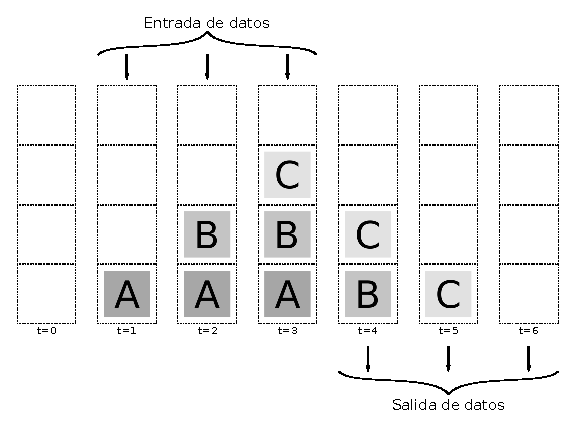
\includegraphics[scale = 0.8]{esquemas/FIFO_bw.eps}
    \caption{Esquema de funcionamiento de una memoria \emph{FIFO}.}
    \label{fig:FIFO_info}
\end{figure}

%* Comprobar
\section{Diseño de un módulo en lenguaje Verilog que actúe como transmisor y receptor serie.}
Se diseñará un módulo que sea capaz de comunicarse bidireccionalmente usando un puerto serie simple\cite{design-uart-vhdl}, pudiendo conectarse a él por medio del circuito integrado FTDI FT2232HL \footnote{Circuito encargado de convertir una conexión \emph{USB High Speed} a dos protocolos configurables distintos. En el caso de la placa de desarrollo \emph{IceStick}, se utiliza un canal para programar la memoria \emph{Flash} SPI utilizada por la \emph{FPGA}, y otro para proporcionar una comunicación UART hacia el equipo.} (disponible en la placa de desarrollo \emph{IceStick}\cite{icestickmanual}), o utilizando un equipo externo compatible.

Por dicho puerto, la \emph{FPGA} transmitirá tanto la trama USB capturada como información del bus, y recibirá los comandos que debe seguir.

En la figura \ref{fig:serie_esquema} se muestra una señal típica serie, esta es la señal que debe ser capturada y generada en la \emph{FPGA}.

\begin{figure}[htb]
    \centering
    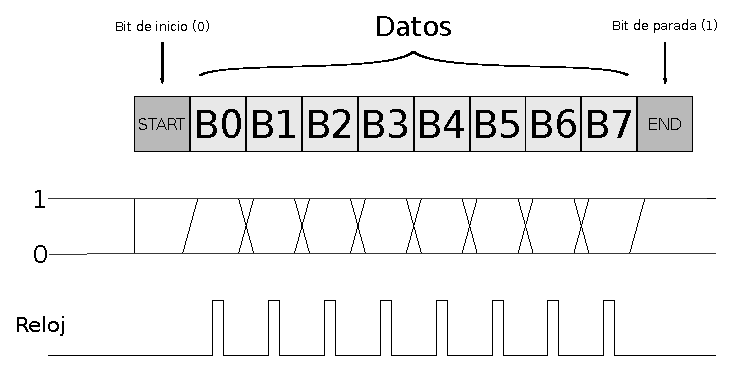
\includegraphics[height=52mm]{esquemas/serie.eps}
    \caption{Señal típica de una comunicación serie.}
    \label{fig:serie_esquema}
\end{figure}

A su vez, este objetivo se puede descomponer en varios subobjetivos.
%* Comprobar
\subsection{Submódulo generador de reloj.}
Este submódulo debe generar un tren de pulsos, a una frecuencia configurable, y con un ancho de pulso igual al del reloj de entrada, permitiendo así trabajar al módulo de comunicación serie a unos baudios deseados.

%* Comprobar
\subsection{Submódulo que cree un registro de desplazamiento universal.}
\label{ssct:registro_desplazamiento}
Submódulo capaz de desplazar tanto a izquierda como a derecha la información almacenada, y que a su vez, permita una carga en paralelo.
La finalidad de este submódulo es poder convertir datos de serie a paralelo o de paralelo a serie, cuando ocurra una recepción o transmisión respectivamente.

En la figura~\ref{fig:shift_ejemplo} se ejemplifica, mostrando sus señales, el funcionamiento de un registro de desplazamiento, en está ocasión, hacia la derecha.

\begin{figure}[htb]
    \centering
    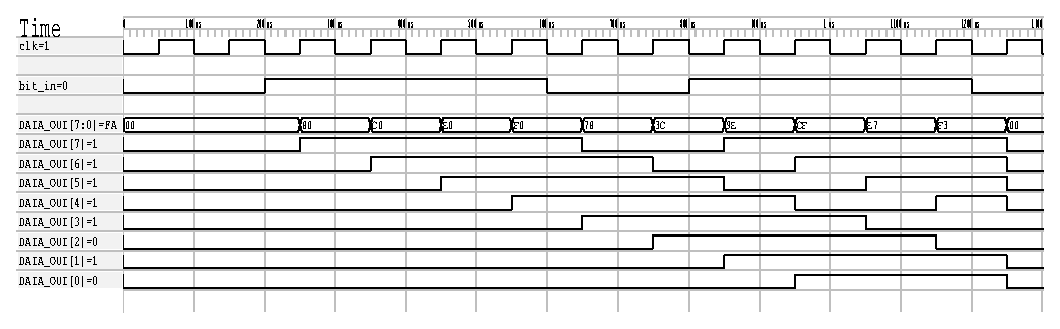
\includegraphics[height=45mm]{esquemas/shift_register.eps}
    \caption{Ejemplo de funcionamiento de un registro de desplazamiento hacia la derecha.}
    \label{fig:shift_ejemplo}
\end{figure}

%* Comprobar
\subsection{Submódulo de emisión serie.}
Submódulo capaz de controlar los datos almacenados en una memoria \emph{FIFO}, para posteriormente transmitirlos por el puerto serie usando el registro de desplazamiento anterior (subsección~\ref{ssct:registro_desplazamiento}).

%* Comprobar
\subsection{Submódulo de recepción serie.}
Submódulo capaz almacenar en una memoria \emph{FIFO} los datos paralelizados capturados en el puerto serie.
% \begin{enumerate}
%     \item \textbf{Submódulo generador de reloj.} \\
%     Este submódulo debe generar un tren de pulsos, a una frecuencia configurable, y con un ancho de pulso igual al del reloj de entrada, permitiendo así trabajar al módulo de comunicación serie a unos baudios deseados.

%     \item \textbf{Submódulo que cree un registro de desplazamiento universal.} \\
%     Submódulo capaz de desplazar tanto a izquierda como a derecha la información almacenada, y que a su vez, permita una carga en paralelo.
%     La finalidad de este submódulo es poder convertir datos de serie a paralelo o de paralelo a serie, cuando ocurra una recepción o transmisión respectivamente.

%     \begin{figure}[htb]
%         \centering
%         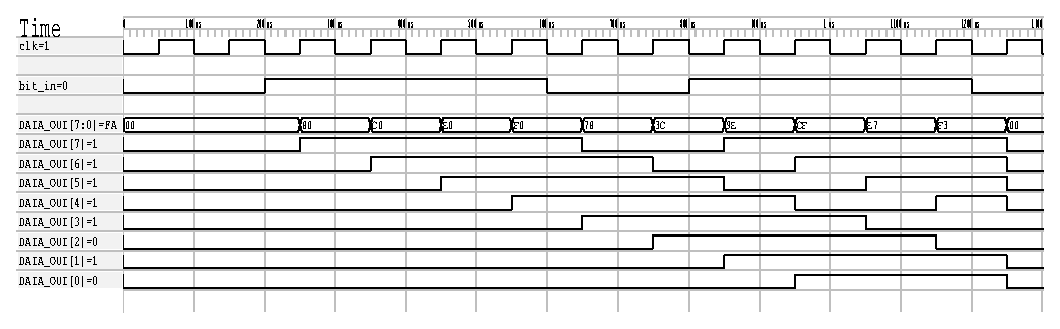
\includegraphics[height=45mm]{esquemas/shift_register.eps}
%         \caption{Ejemplo de funcionamiento de un registro de desplazamiento hacia la derecha.}
%         \label{fig:shift_ejemplo}
%     \end{figure}

%     \item \textbf{Submódulo de emisión serie.} \\
%     Submódulo capaz de controlar los datos almacenados en una memoria \emph{FIFO}, para posteriormente transmitirlos por el puerto serie usando los submódulos anteriores.

%     \item \textbf{Submódulo de recepción serie.} \\
%     Submódulo capaz almacenar en una memoria \emph{FIFO} los datos paralelizados capturados en el puerto serie.
% \end{enumerate}

%! Añadir bib ULPI, USB3300, etc...; Modelo OSI; simbolos megaherzio;
%! Revisar
%! Borrar cosas que sobren??
\section{Diseño de un módulo en lenguaje Verilog que procese el protocolo ULPI.}
Módulo capaz de comunicarse con otros dispositivo compatible con el protocolo ULPI (\emph{UTMI+ Low Pin Interface}), siendo en este caso el integrado USB3300 de \emph{Microchip}, encargado de la capa física USB. \\
El bus utilizado por ULPI consta de una señal de reloj a $60~MHz$ a la que se referencia el resto de señales (\emph{CLK}), 8 señales de datos bidireccionales paralelos (\emph{DATA}), una señal de control de dirección (\emph{DIR}) y dos señales extra de control (\emph{STP} y \emph{NXT}). \\
Debido a que unicamente queremos obtener de forma pasiva los datos USB, de los cuatro posibles modos de funcionamiento ULPI, escritura de registros, lectura de registros, recepción de datos USB y envío de datos USB, solo se van a diseñar los tres primeros. \\
Todas las características y casos del protocolo ULPI están completamente definidas tanto en la hoja de especificaciones del propio protocolo\cite{ulpi-specs} como en la hoja de características del circuito integrado USB3300\cite{microchip:usb3300}.
\begin{enumerate}
    %* Comprobar
    \item \textbf{Submódulo de lectura de registros ULPI} \\
    Submódulo capaz de generar y procesar las señales ULPI necesarias para obtener un valor almacenado en un registro arbitrario del integrado USB3300.
    
    En la figura \ref{fig:ULPI_REG_READ} se puede apreciar la comunicación básica usada para realizar dicha lectura.
    \begin{figure}[htb]
        \centering
        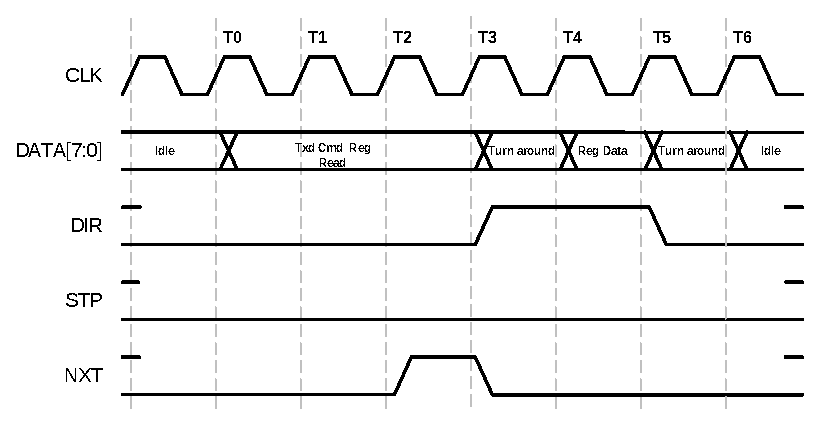
\includegraphics[scale = 0.7]{datasheets/USB3300_REG_READ.eps}
        \caption{Trama de lectura de registros ULPI.}
        \label{fig:ULPI_REG_READ}
    \end{figure}
    
    %* Comprobar
    \item \textbf{Submódulo de escritura de registros ULPI} \\
    Submódulo capaz de generar y procesar las señales ULPI necesarias para almacenar un valor arbitrario de $8~bits$, en un registro del integrado USB3300.
    
    En la figura \ref{fig:ULPI_REG_WRITE} se puede apreciar la comunicación básica usada para realizar dicha escritura.
    \begin{figure}[htb]
        \centering
        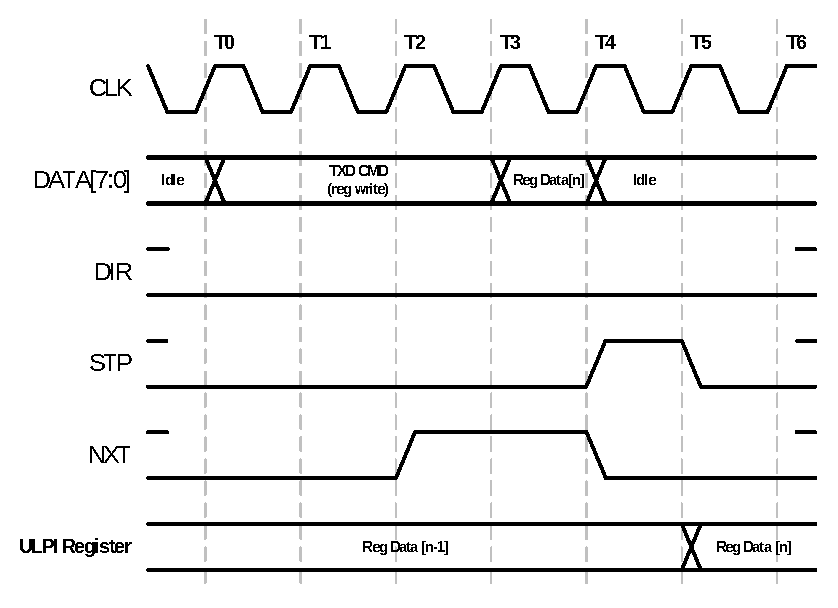
\includegraphics[scale = 0.7]{datasheets/USB3300_REG_WRITE.eps}
        \caption{Trama de escritura de registros ULPI.}
        \label{fig:ULPI_REG_WRITE}
    \end{figure}
    
    %! Revisar
    \item \textbf{Submódulo de captación USB} \\
    Submódulo que ante la llegada de datos USB, sea capaz de procesar las señales ULPI para obtener y clasificar la trama transmitida.
    
    En la figura \ref{fig:ULPI_RECV} se puede apreciar la comunicación básica existente durante la lectura de datos.
    \begin{figure}[htb]
        \centering
        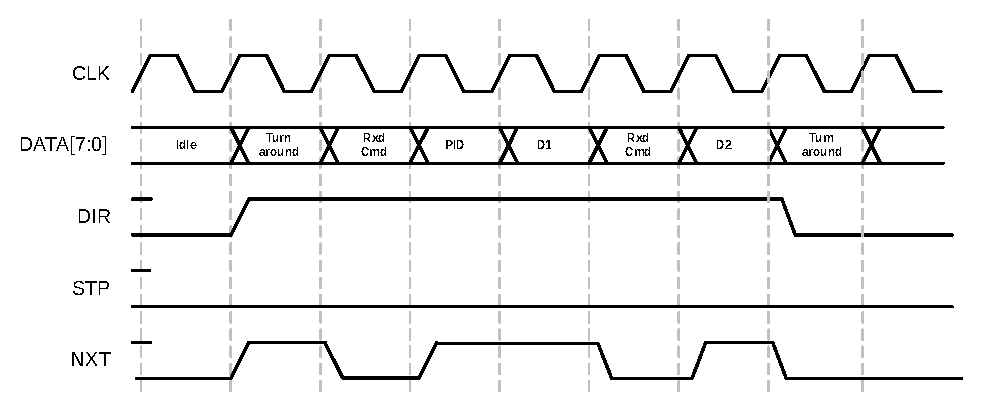
\includegraphics[scale = 0.7]{datasheets/USB3300_RECV.eps}
        \caption{Trama ULPI de recepción de datos USB.}
        \label{fig:ULPI_RECV}
    \end{figure}
\end{enumerate}

%! Revisar
\section{Diseño de un módulo en lenguaje Verilog que gestione los comandos enviados por el usuario.}
Ante cualquier petición realizada por el usuario por el puerto serie, este módulo la procesará obteniendo sus diversas partes (por ejemplo, dirección y datos en una petición de escritura de registro) y las almacenará temporalmente hasta que se puedan ejecutar.

%! Revisar
\section{Diseño de un módulo en lenguaje Verilog que una y gestione todos los módulos.}
Una vez todos los módulos anteriores estén finalizados, es necesaria una sincronización entre ellos que permita obtener el resultado deseado. Por ello, se diseñará un módulo que envíe las señales de control pertinentes al resto de módulos dependiendo de las diversas entradas o registros de control internos.

%! Revisar
\section{Creación de una APP de control en lenguaje C que gestione la comunicación entre el sistema de captura y el equipo.}
Para poder almacenar en el equipo los datos capturados, es necesario crear una aplicación, que por medio de una interfaz básica, permita dar control al usuario varios aspectos del sistema, así como empezar la transmisión de datos al equipo.

%!
\section{Limitaciones generales: FPGA, ULPI, Serie, etc...}




% %! Falta temporización
% \begin{enumerate}
%     %* Comprobar
%     \item \textbf{Diseño de un módulo en lenguaje Verilog que actúe como memoria \emph{FIFO} (siglas en inglés de \emph{First-In First-Out}).} \\
%     Este módulo será capaz de almacenar información de tal forma que el primer dato almacenado sea el primero en ser recuperado. Debido a que la \emph{FPGA} utilizada dispone de 16 bloques de RAM de 4KBits cada uno, se utilizarán varios de estos para no depender unicamente de registros, consiguiendo una mayor capacidad de almacenamiento, con un circuito lo mayor optimizado posible. \\
%     En la figura \ref{fig:FIFO_info} se muestra un esquema del resultado esperado.

%     \begin{figure}[htb]
%         \centering
%         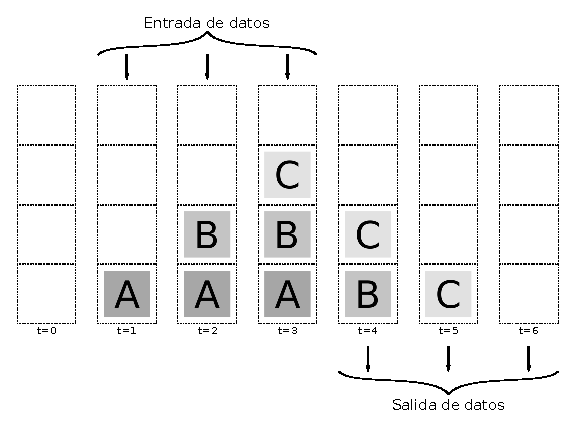
\includegraphics[scale = 0.8]{esquemas/FIFO_bw.eps}
%         \caption{Esquema de funcionamiento de una memoria \emph{FIFO}.}
%         \label{fig:FIFO_info}
%     \end{figure}

%     %! Añadir bib de puerto serie, modos, etc...; FTDI; simbolo baudios;
%     %! Revisar
%     \item \textbf{Diseño de un módulo en lenguaje Verilog que actúe como transmisor y receptor serie.} \\
%     Se diseñará un módulo que sea capaz de comunicarse bidireccionalmente usando un puerto serie simple, pudiendo conectarse a él por medio del circuito integrado FTDI FT2232HL \footnote{Circuito encargado de convertir una conexión \emph{USB High Speed} a dos protocolos configurables distintos. En el caso de la placa de desarrollo \emph{IceStick}, se utiliza un canal para programar la memoria \emph{Flash} SPI utilizada por la \emph{FPGA}, y otro para proporcionar una comunicación UART hacia el equipo.} (disponible en la placa de desarrollo \emph{IceStick}), o utilizando un equipo externo compatible. \\
%     Por dicho puerto, la \emph{FPGA} transmitirá tanto la trama USB capturada como información del bus, y recibirá los comandos que debe seguir. \\
%     Este objetivo se puede descomponer en cuatro subobjetivos:
%     \begin{enumerate}
%         %* Comprobar
%         \item \textbf{Submódulo generador de reloj.} \\
%         Este submódulo debe generar un tren de pulsos, a una frecuencia configurable, y con un ancho de pulso igual al del reloj de entrada, permitiendo así trabajar al módulo de comunicación serie a unos baudios deseados.

%         %* Comprobar
%         \item \textbf{Submódulo que cree un registro de desplazamiento universal.} \\
%         Submódulo capaz de desplazar tanto a izquierda como a derecha la información almacenada, y que a su vez, permita una carga en paralelo.
%         La finalidad de este submódulo es poder convertir datos de serie a paralelo o de paralelo a serie, cuando ocurra una recepción o transmisión respectivamente.

%         %* Comprobar
%         \item \textbf{Submódulo de emisión serie.} \\
%         Submódulo capaz de controlar los datos almacenados en una memoria \emph{FIFO}, para posteriormente transmitirlos por el puerto serie usando los submódulos anteriores.

%         %* Comprobar
%         \item \textbf{Submódulo de recepción serie.} \\
%         Submódulo capaz almacenar en una memoria \emph{FIFO} los datos paralelizados capturados en el puerto serie.
%     \end{enumerate}
    
%     %! Añadir bib ULPI, USB3300, etc...; Modelo OSI; simbolos megaherzio;
%     %! Revisar
%     \item \textbf{Diseño de un módulo en lenguaje Verilog que procese el protocolo ULPI.} \\
%     Módulo capaz de comunicarse con otros dispositivo compatible con el protocolo ULPI (\emph{UTMI+ Low Pin Interface}), siendo en este caso el integrado USB3300 de \emph{Microchip}, encargado de la capa física USB. \\
%     El bus utilizado por ULPI consta de una señal de reloj a 60MHz a la que se referencia el resto de señales (\emph{CLK}), 8 señales de datos bidireccionales paralelos (\emph{DATA}), una señal de control de dirección (\emph{DIR}) y dos señales extra de control (\emph{STP} y \emph{NXT}). \\
%     Debido a que unicamente queremos obtener de forma pasiva los datos USB, de los cuatro posibles modos de funcionamiento ULPI, escritura de registros, lectura de registros, recepción de datos USB y envío de datos USB, solo se van a diseñar los tres primeros. \\
%     Todas las características y casos del protocolo ULPI están completamente definidas tanto en la hoja de especificaciones del propio protocolo\cite{ulpi-specs} como en la hoja de características del circuito integrado USB3300\cite{microchip:usb3300}.
%     \begin{enumerate}
%         %! Revisar
%         \item \textbf{Submódulo de lectura de registros ULPI} \\
%         Submódulo capaz de generar y procesar las señales ULPI necesarias para obtener un valor almacenado en un registro arbitrario del integrado USB3300.
        
%         En la figura \ref{fig:ULPI_REG_READ} se puede apreciar la comunicación básica usada para realizar dicha lectura.
%         \begin{figure}[htb]
%             \centering
%             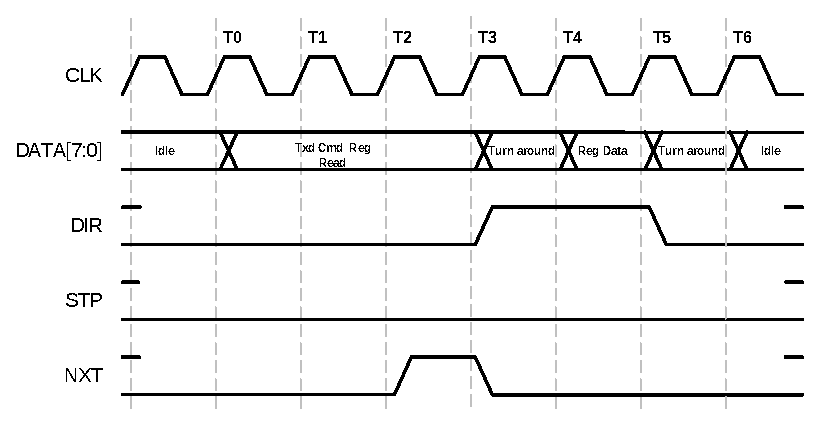
\includegraphics[scale = 0.7]{datasheets/USB3300_REG_READ.eps}
%             \caption{Trama de lectura de registros ULPI.}
%             \label{fig:ULPI_REG_READ}
%         \end{figure}
        
%         %! Revisar
%         \item \textbf{Submódulo de escritura de registros ULPI} \\
%         Submódulo capaz de generar y procesar las señales ULPI necesarias para almacenar un valor arbitrario de 8bits, en un registro del integrado USB3300.
        
%         En la figura \ref{fig:ULPI_REG_WRITE} se puede apreciar la comunicación básica usada para realizar dicha escritura.
%         \begin{figure}[htb]
%             \centering
%             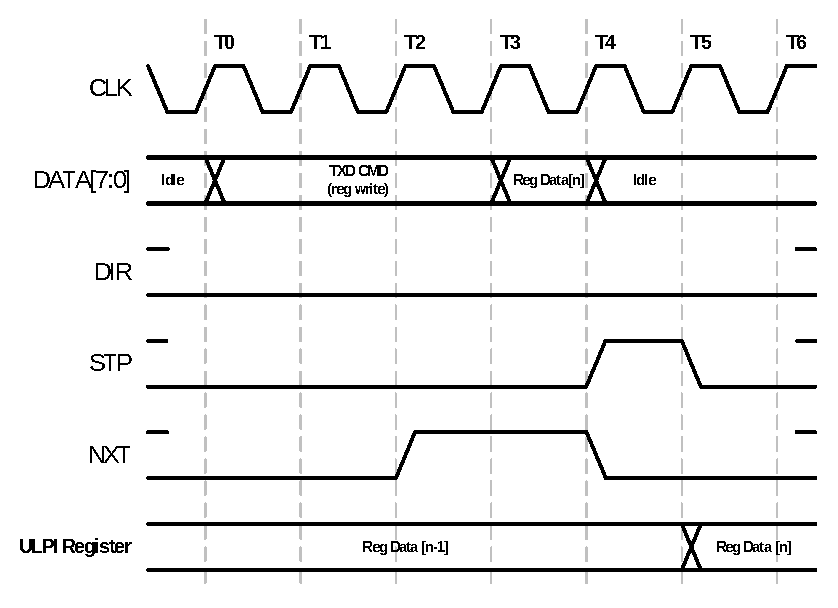
\includegraphics[scale = 0.7]{datasheets/USB3300_REG_WRITE.eps}
%             \caption{Trama de escritura de registros ULPI.}
%             \label{fig:ULPI_REG_WRITE}
%         \end{figure}
        
%         %! Revisar
%         \item \textbf{Submódulo de captación USB} \\
%         Submódulo que ante la llegada de datos USB, sea capaz de procesar las señales ULPI para obtener y clasificar la trama transmitida.
        
%         En la figura \ref{fig:ULPI_RECV} se puede apreciar la comunicación básica existente durante la lectura de datos.
%         \begin{figure}[htb]
%             \centering
%             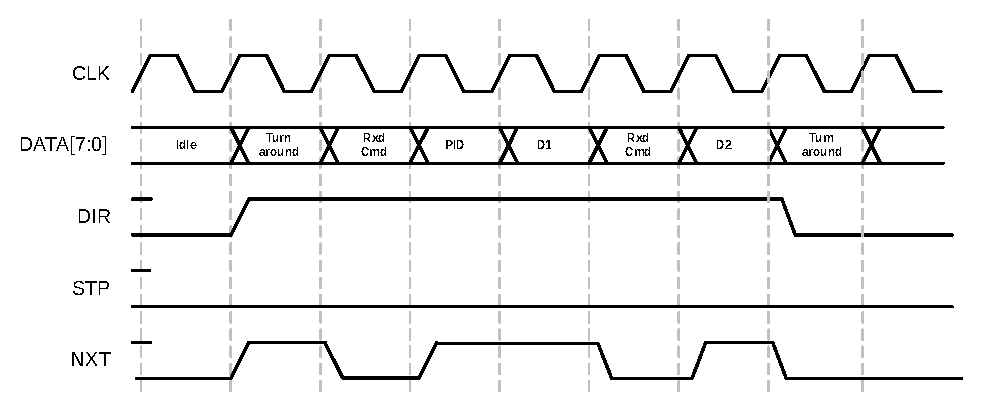
\includegraphics[scale = 0.7]{datasheets/USB3300_RECV.eps}
%             \caption{Trama ULPI de recepción de datos USB.}
%             \label{fig:ULPI_RECV}
%         \end{figure}
%     \end{enumerate}
    
%     %! Revisar
%     \item \textbf{Diseño de un módulo en lenguaje Verilog que gestione los comandos enviados por el usuario.} \\
%     Ante cualquier petición realizada por el usuario por el puerto serie, este módulo la procesará obteniendo sus diversas partes (por ejemplo, dirección y datos en una petición de escritura de registro) y las almacenará temporalmente hasta que se puedan ejecutar.
    
%     %! Revisar
%     \item \textbf{Diseño de un módulo en lenguaje Verilog que una y gestione todos los módulos.} \\
%     Una vez todos los módulos anteriores estén finalizados, es necesaria una sincronización entre ellos que permita obtener el resultado deseado. Por ello, se diseñará un módulo que envíe las señales de control pertinentes al resto de módulos dependiendo de las diversas entradas o registros de control internos.
    
%     %! Revisar
%     \item \textbf{Creación de una APP de control en lenguaje C que gestione la comunicación entre el sistema de captura y el equipo.} \\
%     Para poder almacenar en el equipo los datos capturados, es necesario crear una aplicación, que por medio de una interfaz básica, permita dar control al usuario varios aspectos del sistema, así como empezar la transmisión de datos al equipo.
%     Esta se desarrollará en el lenguaje C, trabajará directamente sobre el puerto serie \footnote{Hará uso de la librería \emph{libserialport} para poder usar los puertos serie. Más información sobre ella en \url{https://sigrok.org/wiki/Libserialport}.}.
% \end{enumerate}

% \chapter{Objetivos}
% \label{ch:objetivos_plantilla}

% Primero enumera los objetivos, no los resumas ni los redactes en un párrafo.  Cada uno de los objetivos de un proyecto debe ser SMART:

% \begin{description}
% \item[Simple] Cada objetivo tiene que ser independiente, tener sentido por sí mismo y más o menos indivisible.  Si no es suficientemente indivisible, pero tiene sentido como una entidad independiente, debes descomponerlo en subobjetivos.
% \item[Medible] Tiene que ser posible medir el grado de consecución al final del TFG.
% \item[Acordado] Los objetivos no los pones tú solo.  Deben partir de un acuerdo con tu director.
% \item[Realista] No pongas objetivos muy ambiciosos. Basta con que resuelva el problema de la forma más simple posible.  Si superas los objetivos nadie se va a quejar.  El director se encargará de que tampoco sean demasiado poco ambiciosos.
% \item[Temporizado] Un objetivo debe tener un marco temporal. Si no es así el objetivo podría no cumplirse nunca.  Es difícil poner límites temporales muy estrictos en un primer proyecto de ingeniería, pero al menos acota.
% \end{description}

% Tras cada objetivo puedes añadir párrafos ampliando la descripción del objetivo, describiendo los límites y justificándolos.  También puedes describir de qué se parte.  Si es posible debería quedar plenamente justificado que se trata de objetivos SMART.  Considera tanto límites intrínsecos (inherentes a la definición del proyecto) como extrínsecos (limitaciones presupuestarias, equipamiento disponible, etc).